\documentclass[oneside,14pt]{extarticle}
\usepackage{cmap}
\usepackage[utf8]{inputenc}
\usepackage{longtable}
\usepackage[english,ukrainian]{babel}
\usepackage{graphicx}
\usepackage{geometry}
\usepackage{listings}
\usepackage{float}
\usepackage{amsmath}
\usepackage{subfig}
\usepackage{tempora}
\renewcommand{\arraystretch}{1.5}
\usepackage{mwe}
\geometry{
	a4paper,
	left=20mm,
	right=20mm,
	top=15mm,
	bottom=15mm,
}
\lstset{
	language=c,
	tabsize=4,
	keepspaces,
	showstringspaces=false,
	frame=single,
	breaklines,
	language=C,
}
\graphicspath{ {./pictures} }
\setlength{\parindent}{4em}

\newcommand\subject{Архітектура і проєктування програмного забезпечення}
\newcommand\lecturer{доцент кафедри ПЗ\\Фоменко А.В.}
\newcommand\teacher{старший викладач кафедри ПЗ\\Шкраб Р.Р.}
\newcommand\mygroup{ПЗ-42}
\newcommand\lab{6}
\newcommand\theme{Використання структурних патернів}
\newcommand\purpose{Ознайомитися з основними шаблонами проектування, навчитися застосовувати їх при проектуванні і розробці ПЗ}

\begin{document}
\begin{normalsize}
	\begin{titlepage}
		\thispagestyle{empty}
		\begin{center}
			\textbf{МІНІСТЕРСТВО ОСВІТИ І НАУКИ УКРАЇНИ\\
				НАЦІОНАЛЬНИЙ УНІВЕРСИТЕТ "ЛЬВІВСЬКА ПОЛІТЕХНІКА"}
		\end{center}
		\begin{flushright}
			\textbf{ІКНІ}\\
			Кафедра \textbf{ПЗ}
		\end{flushright}
		\vspace{80pt}
		\begin{center}
			\textbf{ЗВІТ}\\
			\vspace{10pt}
			до лабораторної роботи № \lab\\
			\textbf{на тему}: <<\textit{\theme}>>\\
			\textbf{з дисципліни}: <<\subject>>
		\end{center}
		\vspace{80pt}
		\begin{flushright}
			
			\textbf{Лектор}:\\
			\lecturer\\
			\vspace{28pt}
			\textbf{Виконав}:\\
			
			студенти групи \mygroup\\
			Коваленко Д.М.\\
			Снісар В.І.\\
			Баран В.Б.\\
			\vspace{28pt}
			\textbf{Прийняла}:\\
			
			\teacher\\
			
			\vspace{28pt}
			«\rule{1cm}{0.15mm}» \rule{1.5cm}{0.15mm} 2024 р.\\
			$\sum$ = \rule{1cm}{0.15mm}……………\\
			
		\end{flushright}
		\vspace{\fill}
		\begin{center}
			\textbf{Львів — 2024}
		\end{center}
	\end{titlepage}
		
	\begin{description}
		\item[Тема.] \theme.
		\item[Мета.] \purpose.
	\end{description}

    \section*{Лабораторне завдання}
    \begin{enumerate}
    	\item Вивчити поведінкові патерни. Вивчити породжаючі патерни. Вивчити структурні патерни , описати можливість використання 2-х патернів у розробляємому модулі.
    	\item Продемонструвати на діаграмі класів.
    	\item Навести або код, або псевдокод.
    	\item Описати і продемонструвати хоча б один архітектурний патерн.
    \end{enumerate}
    
    \section*{Хід роботи}
    \subsection*{Можливість використання патернів у розробляємому модулі}
    У модулі проектування для віртуальної лабораторії можна використати кілька шаблонів проектування, що підвищать модульність, гнучкість і підтримуваність системи. Розглянемо популярний шаблон, що може бути корисними в цьому контексті: Decorator.
    
    \subsection*{Декоратор}
    Декоратор — це патерн проєктування, що дозволяє динамічно додавати об’єкту нові функції, не змінюючи його структуру. У коді, який ви надаєте, цей патерн використовується для надання елементам UML діаграм різних властивостей залежно від режиму або стану додатку.
    
    \subsection*{Діаграма класів}
    \begin{figure}[H]
    	\centering
    	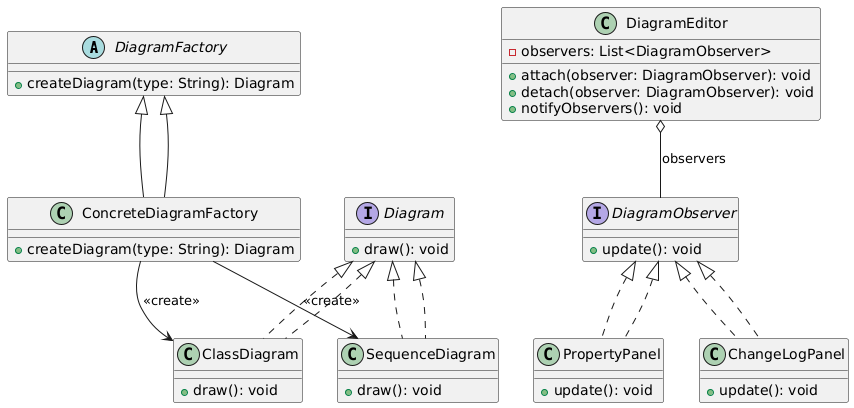
\includegraphics[width=\columnwidth]{1}
    	\caption{Декоратор}
    \end{figure}
    \begin{small}
    	\begin{lstlisting}
const features = { ...UMLElements, ...UMLRelationships }[props.type].features as UMLElementFeatures &
UMLRelationshipFeatures;
const component = props.type in UMLRelationshipType ? CanvasRelationship : CanvasElement;
const decorators = [];

if (props.mode === ApollonMode.Assessment) {
decorators.push(assessable, updatable, selectable, hoverable);
} else if (props.readonly) {
decorators.push(selectable, hoverable);
} else if (props.view === ApollonView.Exporting || props.view === ApollonView.Highlight) {
decorators.push(interactable, hoverable);
} else if (props.view === ApollonView.Modelling) {
if (props.features.hoverable && features.hoverable) {
	decorators.push(hoverable);
}
if (features.reconnectable) {
	decorators.push(reconnectable);
}
if (props.features.selectable && features.selectable) {
	decorators.push(selectable);
}
if (props.features.movable && features.movable) {
	decorators.push(movable);
}
if (props.features.resizable && features.resizable) {
	const options = {
		preventY: features.resizable === 'WIDTH',
		preventX: features.resizable === 'HEIGHT',
	};
	decorators.push(resizable(options));
}
if (props.features.connectable && features.connectable) {
	decorators.push(connectable);
}
if (props.features.updatable && features.updatable) {
	decorators.push(updatable);
}
if (props.features.droppable && features.droppable) {
	decorators.push(droppable);
}
}

type Compose = ConnectedComponent<
ComponentType<
UMLElementComponentProps & {
child: React.ComponentClass<any>;
}
>,
any
>;

// reverse, because compose creates one function by composing the given functions from right to left
return {
component: compose<Compose>(...decorators.reverse())(component),
};
    	\end{lstlisting}
    \end{small}
    
    
    \begin{enumerate}
    	\item \textbf{Ініціалізація компонентів та функцій:}
    	\begin{itemize}
    		\item Спочатку визначається об'єкт \texttt{features}, що комбінує властивості \texttt{UMLElements} та \texttt{UMLRelationships} в залежності від типу елемента (вказаного в \texttt{props.type}).
    		\item Залежно від цього типу обирається відповідний компонент: \textit{CanvasRelationship} або \textit{CanvasElement}.
    	\end{itemize}
    	
    	\item \textbf{Вибір декораторів залежно від умов:}
    	\begin{enumerate}
    		\item Якщо режим \texttt{props.mode} є \texttt{Assessment}, додаються декоратори:
    		\begin{itemize}
    			\item \texttt{assessable}
    			\item \texttt{updatable}
    			\item \texttt{selectable}
    			\item \texttt{hoverable}
    		\end{itemize}
    		\item Якщо \texttt{props.readonly} дорівнює \texttt{true}, додаються:
    		\begin{itemize}
    			\item \texttt{selectable}
    			\item \texttt{hoverable}
    		\end{itemize}
    		\item Якщо \texttt{props.view} має значення \texttt{Exporting} або \texttt{Highlight}, додаються:
    		\begin{itemize}
    			\item \texttt{interactable}
    			\item \texttt{hoverable}
    		\end{itemize}
    		\item Якщо \texttt{props.view} дорівнює \texttt{Modelling}, додаються декоратори в залежності від властивостей:
    		\begin{itemize}
    			\item \texttt{hoverable} (якщо \texttt{features.hoverable} активне)
    			\item \texttt{reconnectable} (якщо доступно)
    			\item \texttt{movable} (якщо доступно)
    			\item \texttt{resizable} (з параметрами, якщо доступно)
    			\item \texttt{connectable} (якщо доступно)
    			\item \texttt{updatable} (якщо доступно)
    			\item \texttt{droppable} (якщо доступно)
    		\end{itemize}
    	\end{enumerate}
    	
    	\item \textbf{Композиція декораторів:}
    	\begin{itemize}
    		\item Використовується функція \texttt{compose} для композиції декораторів у зворотному порядку. Всі декоратори додаються до компонента, створюючи новий компонент з усіма необхідними властивостями.
    	\end{itemize}
    \end{enumerate}
    
	\section*{Висновки}
	У ході виконання лабораторної роботи ми ознайомилися з основними шаблонами проектування, навчилися застосовувати їх при проектуванні і розробці ПЗ.

	    
\end{normalsize}
\end{document}
